%%%%%%%%%%%%%%%%%%%%%%%%%%%%%%%%%%%%%%%%%%%%%%%%%%%%%%%
% % Lines starting with % are comments, which are ignored.
% % This is a handy way of indicating the date and version of
% % your document, to wit:
% %
% % LaTeX sample file
% % Modified March, 2002
% %
%%%%%%%%%%%%%%%%%%%%%%%%%%%%%%%%%%%%%%%%%%%%%%%%%%%%%%%
\DocumentMetadata{
  % PDF standards: ONE key whose value is a comma-separated list --
  % UA-2 (accessibility) plus A-4f (archival; the archival companion of
  % UA-2). Do NOT use separate pdfstandard=... keys: with ordinary
  % key-value parsing only the last one takes effect.
  pdfstandard={UA-2,A-4f},
  lang=en-US,
  tagging=on,
  tagging-setup={
    math/setup=mathml-SE
  }
}

\documentclass{ltx-talk}
% lecture-macros.tex -- shared package setup for lecture-template.tex
% (ltx-talk slides / handouts).
%
% NOTE ON PATHS: every template in this repository is stored one level up
% from where it is compiled (see README.md). All relative \input paths
% below are resolved against the folder the document is compiled in,
% which sits one directory above this file.

% --- Tables, bookmarks, strikethrough ------------------------------------
% booktabs: professional table rules (\toprule, \midrule, \bottomrule)
% bookmark: PDF outline entries (PDF bookmarks)
% ulem[normalem]: \sout strikethrough that survives math mode
\usepackage{booktabs}
\usepackage{bookmark}
\usepackage[normalem]{ulem}
\usepackage{multicol}

% --- Math ------------------------------------------------------------
% amsmath: equation environments and numbering
% mathrsfs: \mathfrak  |  stmaryrd: extra symbols
\usepackage{amsmath}
\usepackage{mathrsfs}
\usepackage{stmaryrd}

% --- Layout -------------------------------------------------------------
% float: [H] float placement
% fontspec: Unicode/OpenType fonts (compile with XeLaTeX or LuaLaTeX)
\usepackage{float}
\usepackage{fontspec}

% --- Colors ---------------------------------------------------------------
% dvipsnames: extended named color palette (the Accessible* colors below
% are built on it);
% table: \rowcolors / \cellcolor for shading tables.
% NOTE: xcolor may only be loaded ONCE per document -- a second
% \usepackage{xcolor} with different options is a fatal "Option clash"
% error, so ALL of its options are listed here.
\usepackage[dvipsnames,table]{xcolor}

% --- Multimedia -----------------------------------------------------------
% animate: embeds audio/video (and legacy Flash) media in a frame.
\usepackage{animate}

% --- Bibliography ----------------------------------------------------------
% biblatex (biber backend): citations for lecture notes.
\usepackage[
  backend=biber,
  style=alphabetic,
  url=true,
  doi=true,
  isbn=true,
  backref=true
]{biblatex}

% --- Colored boxes ----------------------------------------------------------
% talkthemetcolorbox: the colored-box theme for ltx-talk slides
% (shadow/rounded/shaded blocks, showtitle, titlepage styles).
\usepackage[
  shadow,
  rounded,
  shaded,
  blocks,
  showtitle,
  titlepage
]{talkthemetcolorbox}

% --- "theindex" helper environment ------------------------------------------
% Provides a lightweight theindex environment (an itemize) and the
% \@idxitem/\subitem/\subsubitem/\indexspace macros that LaTeX's standard
% theindex machinery expects, so hand-written index pages indent correctly.
\makeatletter
\newenvironment{theindex}
  {\begin{itemize}}
  {\end{itemize}}
\providecommand\@idxitem{\par\hangindent 40\p@}
\providecommand\subitem{\@idxitem \hspace*{20\p@}}
\providecommand\subsubitem{\@idxitem \hspace*{30\p@}}
\providecommand\indexspace{\par \vskip 10\p@ \@plus5\p@ \@minus3\p@\relax}
\makeatother

% --- Index -----------------------------------------------------------------
% imakeidx: builds the printed index.
% The redefinition below appends "|hyperpage" to every index entry so that,
% in the PDF, each index entry is a link to its page.
\usepackage{imakeidx}
\makeatletter
\let\imki@orig@wrindexentrysplit\imki@wrindexentrysplit
\renewcommand\imki@wrindexentrysplit[3]{%
  \imki@orig@wrindexentrysplit{#1}{#2|hyperpage}{#3}%
}

\makeatletter
% --- Section titles: capture + one bookmark per logical section -------------
% \section is redefined so that:
%   1. the section title is captured into the plain-TeX register
%      \mytalksectitletoks (reprinted verbatim on the auto divider frame,
%      see the cmd/section/after hook below -- plain-TeX storage is
%      catcode-safe, unlike expanding the title in a hook), and
%   2. exactly ONE depth-1 PDF bookmark is created per \section call
%      (hyperref's own bookmark is suppressed via \Hy@writebookmark).
\DeclareCommandCopy{\OriginalSectionForBookmarks}{\section}
\newtoks\mytalksectitletoks

\RenewDocumentCommand{\section}{s o m}{%
  \begingroup
    \def\Hy@writebookmark##1##2##3##4##5{}%
    \global\mytalksectitletoks={#3}%
    \IfBooleanTF{#1}
      {\phantomsection\IfNoValueTF{#2}{\OriginalSectionForBookmarks*{#3}}{\OriginalSectionForBookmarks*[#2]{#3}}}%
      {\IfNoValueTF{#2}{\OriginalSectionForBookmarks{#3}}{\OriginalSectionForBookmarks[#2]{#3}}}%
  \endgroup
  \IfBooleanTF{#1}
    {\IfNoValueTF{#2}{\pdfbookmark[1]{#3}{section-star.\thepage.\number\inputlineno}}{\pdfbookmark[1]{#2}{section-star.\thepage.\number\inputlineno}}}%
    {\IfNoValueTF{#2}{\pdfbookmark[1]{Section \thesection: #3}{section.\thesection}}{\pdfbookmark[1]{Section \thesection: #2}{section.\thesection}}}%
}
\makeatother

% --- One PDF bookmark per logical frame (NOT per overlay) ---------------------
% ltx-talk writes one PDF page per overlay, so a naive frametitle hook would
% register a new bookmark for every overlay of the same frame. The
% \g_slideutils_frame_bookmark_int register remembers the last frame that
% got a bookmark, so subsequent overlays of the same frame are skipped.
% This is also what keeps BeamerPresenter's cumulative annotations working:
% one logical frame must stay one logical unit in the PDF outline.
\ExplSyntaxOn
\int_new:N \g_slideutils_frame_bookmark_int

\AddToHook{cmd/frametitle/after}{%
  \tl_if_empty:NF \g__talk_frame_title_tl
    {
      \ifnum\value{frame}=\g_slideutils_frame_bookmark_int\relax
      \else
        \int_gset:Nn \g_slideutils_frame_bookmark_int { \value{frame} }%
        \pdfbookmark[2]{\tl_use:N \g__talk_frame_title_tl}
          {frame.\int_use:N \g_slideutils_frame_bookmark_int}
      \fi
    }
}
\ExplSyntaxOff
\makeatother

% --- Printed index + theme for the colored boxes -------------------------------
% \makeindex[...]: two-column index titled "Index", listed in the TOC.
% The two EditInstance calls style the standard header/footer instances
% of talkthemetcolorbox (cyan background; footer order title/author/
% date/framenumber).
\makeindex[columns=2, title=Index, intoc]\EditInstance{header}{std}{
  background-color = cyan,
  color            = black,
  height           = 0.75cm
}
\EditInstance{footer}{std}{
  background-color = cyan,
  element-order = {title, author, date, framenumber},
}

% --- Auto section divider frame ---------------------------------------------------
% After each \section, insert a centered, large, structure-colored frame
% that prints the section title (from \mytalksectitletoks).
\AddToHook{cmd/section/after}{%
  \begin{frame}
    \centering
    \color{structure}
    \LARGE
    \the\mytalksectitletoks
  \end{frame}%
}

% --- Tagging sockets (tagged PDF structure) ---------------------------------------
% ltx-talk exposes tagging "sockets" where the PDF structure can attach
% section titles; register one and leave it unassigned (none) so the
% class's own tagging keeps control.
\ExplSyntaxOn
\AtBeginDocument{
  \NewTaggingSocketPlug { talk / sec / title } { none } { }
  \AssignTaggingSocketPlug { talk / sec / title } { none }
}
\ExplSyntaxOff

% --- Accessibility roles ----------------------------------------------------------------
% Map \frametitle to the H1 heading role in the tagged PDF, so screen
% readers treat slide titles as headings.
\tagpdfsetup{role / new-tag = frametitle / H1}

\makeatletter
% --- Page label = frame number -------------------------------------------------------
% Redefine what feeds the PDF page label to track the frame counter,
% not the physical page counter. Replace \theframenumber below with
% whatever internal macro/property ltx-talk actually uses to produce
% the "framenumber" footer element — confirm via ltx-talk-frame.dtx.
\renewcommand\thepage{\arabic{frame}}
\makeatother

\addbibresource{refs.bib}

% --- "Problem Time!" slides ------------------------------------------------------------------
% \ProblemSlide{problem}{solution} emits two frames: the problem, then
% its solution after a \pause, each numbered by the problem counter.
\newcounter{problemcounter}
\setcounter{problemcounter}{0}
\newcommand{\ProblemSlide}[2]{
  \stepcounter{problemcounter}
  \begin{frame}
    \frametitle{Problem Time!}
    Problem \theproblemcounter: #1
  \end{frame}

  \begin{frame}
    \frametitle{Problem Time!}
    Solution to Problem \theproblemcounter: \pause

    #2
  \end{frame}
}
% \highlight[<colour>]{<stuff>}
% from https://tex.stackexchange.com/questions/33401/a-version-of-colorbox-that-works-inside-math-environments
\newcommand{\highlight}[2][yellow]{\mathchoice%
  {\colorbox{#1}{$\displaystyle#2$}}%
  {\colorbox{#1}{$\textstyle#2$}}%
  {\colorbox{#1}{$\scriptstyle#2$}}%
  {\colorbox{#1}{$\scriptscriptstyle#2$}}}%

% --- Fonts ------------------------------------------------------------------------------
% Lato (text) + LeteSansMath (math): open, accessible typefaces.
\setmainfont{Lato}[
  Ligatures=TeX,
  Numbers={Lining,Monospaced}
]
\setsansfont{Lato}[
  Ligatures=TeX,
  Numbers={Lining,Monospaced}
]
\setmathfont{LeteSansMath.otf}\usepackage{emoji}

% --- Accessible colors ---------------------------------------------------------------------
% WCAG-contrast-safe variants of red/green for text on white:
% red!80!black and green!40!black both clear the 4.5:1 requirement.
% AltYellow: soft background for highlight boxes.
\colorlet{AccessibleRed}{red!80!black}
\colorlet{AccessibleGreen}{green!40!black}
\definecolor{AltYellow}{RGB}{255,245,170}

% --- Links ---------------------------------------------------------------------------------
% hyperref + link colors: every link uses AccessibleGreen (7.2:1 on
% white), so internal, citation, and URL links all pass WCAG 1.4.3.
\usepackage{hyperref}
\hypersetup{
  colorlinks=true,
  linkcolor=AccessibleGreen,
  urlcolor=AccessibleGreen,
  citecolor=AccessibleGreen,
}

% --- Shared course macros ---------------------------------------------------------------------
% Root macros.tex: math shorthands used across all course documents
% (\RR, \NN, \ZZ, \QQ, \grad, \curl, \tr, \der, \pder, ...).
\newcommand{\RR}{\mathbb{R}}
\newcommand{\NN}{\mathbb{N}}
\newcommand{\ZZ}{\mathbb{Z}}
\newcommand{\QQ}{\mathbb{Q}}
\newcommand{\vv}{\vec{v}}
\newcommand{\ww}{\vec{w}}
\newcommand{\xx}{\vec{x}}
\newcommand{\yy}{\vec{y}}
\newcommand{\zz}{\vec{z}}
\newcommand{\uu}{\vec{u}}
\newcommand{\basis}[1]{\vec{e_{#1}}}
\newcommand{\id}{\mathrm{id}}
\newcommand{\CC}{\mathbb{C}}
\renewcommand{\div}{\operatorname{div}}
\newcommand{\grad}{\operatorname{grad}}
\newcommand{\curl}{\operatorname{curl}}
\newcommand{\tr}{\operatorname{tr}}
\newcommand{\der}[2]{\dfrac{d #1}{d #2}}
\newcommand{\pder}[3][]{\dfrac{\partial^{#1} #2}{\partial #3}}


% % Title and author(s)
%%%%%%%%%%%%%%%%%%%%%%%%%%%%%%%%%%%%%%%%%%%%%%%%%%%%%%%
\title{Lecture 2: Introduction to Limits}
\author{Garrett Credi}
\date{09/10/2026}
%%%%%%%%%%%%%%%%%%%%%%%%%%%%%%%%%%%%%%%%%%%%%%%%%%%%%%%
% %
% % The next command allows your in import encapsulated
% % postscript files, .epsf or .eps files, which
% % contain vector graphic image data.
% %
%%%%%%%%%%%%%%%%%%%%%%%%%%%%%%%%%%%%%%%%%%%%%%%%%%%%%%%
% %   The first thanks indicates your affiliation
% %
% %  Just the name here.
% %
% % Your mailing address goes at the end.
% %
% % \thanks is also how you indicate grant support
% %
%%%%%%%%%%%%%%%%%%%%%%%%%%%%%%%%%%%%%%%%%%%%%%%%%%%%%%%

%%%%%%%%%%%%%%%%%%%%%%%%%%%%%%%%%%%%%%%%%%%%%%%%%%%%%%%
% $ The next command ensures the margins are 1 inch on
% % all sides.
% %
%%%%%%%%%%%%%%%%%%%%%%%%%%%%%%%%%%%%%%%%%%%%%%%%%%%%%%%
\begin{document}
\begin{frame}
  \maketitle
\end{frame}

\begin{frame}
  \frametitle{Day 1 Recap}

  Questions: \pause
  \begin{enumerate}
    \item Was everyone able to access the Gradescope/homework? \pause
    \item How did the homework go? (Note: Length will not be as long for future HWs, this one just had a lot of topics to review) \pause
    \item Any questions, comments, concerns?
  \end{enumerate}
\end{frame}

\begin{frame}
  \frametitle{Quiz Time!}

  At this point it's quiz time! \pause

  \begin{enumerate}
    \item Get into neatly organized rows
    \item Do not flip over the page and start until directed to
    \item Should go without saying but no cheating!
      \begin{itemize}
        \item No looking at neighbors papers
        \item No calculators
        \item No notes
        \item No phones
        \item etc. etc.
      \end{itemize}
    \item I'll write on the board the minutes you have left, crossing each number out when you have \textit{less than} that number of minutes left to complete
    \item When time is up, stop writing and hold your quiz up so I can grab it. If you finish early, just chill until the 5 mins are up.
  \end{enumerate}
\end{frame}

\begin{frame}
  \frametitle{Time to do some math!}

  Now let's start the lecture!
\end{frame}

\section{Limits}

\begin{frame}
  \frametitle{MATH 1271 - Part 1: Limits}

  We will start our course by discussing the concept of a \textit{limit of a function}. \pause

  Intuitively, the limit serves several important purposes: \pause
  \begin{itemize}
    \item It gives you information about the value that a function tends towards,
      as it's input tends towards some fixed input. \pause
    \item It tells you what value the function is ``approximating" around some fixed input.\pause
    \item It tells you local information about the function around some \textit{small neighborhood} of some fixed input.
  \end{itemize}
\end{frame}

\subsection{Approximation}
\begin{frame}
  \frametitle{Approximation I}

  Let's run with the second interpretation for a bit: \pause

  Say you're doing some experiment where you're studying the relationship between \pause
  some \textit{input variable} $x$ (maybe it's the concentration of some acid in a solution) \pause
  and some \textit{output variable} $y$ (maybe it's the pH of that solution). \pause

  Real world problems: \pause
  \begin{enumerate}
    \item We can almost never perfectly measure physical quantities e.g.
      \begin{enumerate}
        \item We can't know the exact number of molecules of an acid present in a solution, only up to some error \pause
        \item Using typical measurements like pH strips etc. we also can't get a precise measurement of the output variable either \pause
      \end{enumerate}
  \end{enumerate}

  How do we proceed if, for instance, we want to know the \textit{exact} pH of a solution
  whose concentration of acid is \textit{exactly} 0.5 moles per liter?
\end{frame}

\begin{frame}
  \frametitle{Approximation II}

  We can either: \pause
  \begin{enumerate}
    \item Make \text{many many many} measurements and take their average, or \pause
    \item Use more precise methods of measurements that decrease the error range as much as possible. \pause
  \end{enumerate}

  Graphically: \vspace{\stretch{1}}
\end{frame}

\begin{frame}
  \frametitle{Approximation III}

  \begin{alertblock}{WARNING!}
    How do we actually know that this average we're taking is the true output value?
  \end{alertblock} \pause

  What it really is, is... \pause

  The Limit!
\end{frame}

\begin{frame}
  \frametitle{Limits I}

  \begin{block}{Limit of a Function}\index{limit}
    For some function $f : \RR \rightarrow \RR$ and some fixed input $x_0 \in \RR$, \pause
    we say that $\lim_{x \rightarrow x_0} f(x) = L$ (said ``the limit of $f(x)$ as $x$ approaches $x_0$ is $L$") \pause
    if we can make $f(x)$ as close to $L$ as we want just by forcing $x$ to be close enough to $x_0$. \pause

    Explicitly: for any error tolerance $\epsilon > 0$, if we want $f(x)$ to be equal to $L$
    within an error of $\epsilon$ (e.g. $|f(x) - L| <  \epsilon$), \pause then we just need to find some 
    input error tolerance $\delta > 0$ and ensure that $x$ is equal to $x_0$ within an error of $\delta$ (e.g. $|x - x_0| < \delta$).

    If no such value $L$ exists \pause (i.e. the function \textit{cannot} be well approximated around $x_0$) \pause
    then we say that $\lim_{x \rightarrow x_0} f(x)$ \textit{does not exist}. \index{limit!does not exist}
  \end{block}
\end{frame}

\begin{frame}
  \frametitle{Limits II}

  How can we find limits? \pause

  Option 1 (easiest): Graphically! \pause

  Given a graph of a function, we can easily tell what value a function approaches
  \pause just by examining where the graph tends towards as we near a given point.

  \begin{figure}[htpb]
    \centering
    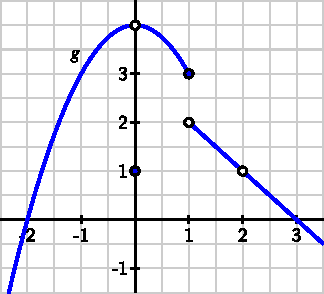
\includegraphics[height=0.5\textheight,alt={A function with a hole discontinuity at $0$ and $2$, and a jump discontinuity at $1$}]{./1_2_PA1.pdf}
    \caption{An example function}
  \end{figure}
\end{frame}

\begin{frame}
  \frametitle{Limits III}

  What if we don't have a graph to work with? \pause

  Option 2 (medium easy, \textit{only an estimate!}): Evaluation! \pause

  Given an expression of a function, e.g. $f(x) = x^2$ \pause and a specific
  value around which to compute the limit, e.g. $x_0 = 2$, \pause
  we can compute values that are closer and closer to $x_0$ \textit{by hand/calculator} \pause
  and guess if they're approaching a value. \pause (Similar to the method we talked about in the approximation section.)

  \vspace{\stretch{0.8}}
\end{frame}

\begin{frame}
  \frametitle{Limits IV}

  What about if we are both: \pause
  \begin{enumerate}
    \item Not given a graph \pause
    \item Interested in the \textit{exact} limit, not an approximation? \pause
  \end{enumerate}

  Option 3 (exact!): Algebraic Manipulation! \pause

  E.g., if we wanted to find $\lim_{x \rightarrow 2} x^2$ we could: \pause

  \begin{enumerate}
    \item Rewrite it as $\lim_{h \rightarrow 0} (2 + h)^2$ \pause
    \item Expand the argument to get $\lim_{h \rightarrow 0} 4 + 2h + h^2$ \pause
    \item Group the $h$ terms together to get $\lim_{h \rightarrow 0} 4 + h(2 + h)$ \pause
    \item Notice that as $h \rightarrow 0$, \pause $h(2+h) \rightarrow 0$ as well so $\lim_{x \rightarrow 2} x^2 = 4$
  \end{enumerate}
\end{frame}

\begin{frame}
  \frametitle{Limits V}

  Notice that $\lim_{x \rightarrow 2} x^2 = 4 = 2^2 = f(2)$ \pause
  i.e. \textit{the limit of $f(x)$ as $x \rightarrow x_0$ is equal to $f(x_0)$}! \pause

  Is this always true? \pause I.e. no matter what function $f$ we choose and what fixed input $x_0$ we take, \pause
  do we always have that: 
  \begin{equation}
    \lim_{x \rightarrow x_0} f(x) \stackrel{?}{=} f(x_0)
  \end{equation} \pause
\end{frame}
\begin{frame}
  \frametitle{Limits VI}
  \begin{alertblock}{NO!}
    Two things can go wrong: \pause
    \begin{enumerate}
      \item We can artifically redefine the value of a function as much as we want: \pause
        \begin{equation}
          f(x) = \begin{cases} 4, & x = 0 \\ x^2, & x \neq 0 \end{cases}
        \end{equation} \pause
      \item We can have a function that isn't \textit{defined} at a point but still \textit{has a limit at that point}: \pause
        \begin{equation}
          g(x) = \dfrac{x^2 - 1}{x + 1}.
        \end{equation}
    \end{enumerate}
  \end{alertblock}
\end{frame}
\begin{frame}
  \frametitle{Limits VII}
  Let's study that $g(x) = \dfrac{x^2 - 1}{x + 1}$ function more: \pause

  \begin{enumerate}
    \item What is the domain of $g$? \pause
    \item For points $x_0$ in the domain of $g$, is it true that $\lim_{x \rightarrow x_0} g(x) = g(x_0)$? \pause
    \item What about the point that is \textit{not} in the domain of $g$? What is $\lim_{x \rightarrow -1} g(x)$?
  \end{enumerate}

  \vspace{\stretch{0.6}}
\end{frame}

\begin{frame}
  \frametitle{Limits VIII}
  Let's try another weird function: \pause
  \begin{equation}
    h(x) = \sin(\dfrac{\pi}{x}).
  \end{equation} \pause

  \begin{enumerate}
    \item Domain? \pause
    \item Does limit=value for points in the domain? \pause
    \item What about $x_0 = 0$?
  \end{enumerate}
\end{frame}

\begin{frame}
  \frametitle{Instantaneous Velocity I}

  What can we \textit{do} with limits? \pause

  \begin{block}{Average Velocity}\index{average velocity}\index{velocity!average}
    Suppose that an object's position as a function of time $t$
    is given by the function $s(t)$. \pause

    The average velocity of the object, from time $t = a$ to time $t = b$
    is given by: \pause
    \begin{equation}
      AV_{[a, b]} := \dfrac{s(b) - s(a)}{b - a}.
    \end{equation} \pause
  \end{block}

  However, we rarely ever see \textit{average} velocity in real life! \pause
  E.g. if you drive a car then the dashboard reports your speed exactly
  in the instant you look at it, not over the last 1, 2, 5, etc. minutes! \pause

  (If it did, imagine someone driving slowly for a while, 
  rapidly accelerating to a dangerous speed,
  getting pulled over and then trying to tell the cop
  ``oh well my car said my average speed over the past 5 minutes was just 20mph"
  unlikely to avoid a ticket!)
\end{frame}

\begin{frame}
  \frametitle{Instantaneous Velocity II}
  That why we care about the \textit{instantaneous} velocity of an object: \pause

  \begin{block}{Instantaneous Velocity}\index{instantaneous velocity}\index{velocity!instantaneous}
    Suppose that an object's position as a function of time $t$
    is given by the function $s(t)$. \pause

    The instantaneous velocity of the object at time $t = a$ is defined as \pause
    \begin{equation}
      IV_{t = a} = \lim_{\Delta t \rightarrow 0} AV_{[a, a + \Delta t]} = \lim_{h \rightarrow 0} \dfrac{s(a + h) - s(a)}{h}
    \end{equation}
  \end{block}
\end{frame}

\begin{frame}
  \frametitle{Instantaneous Velocity III}
    
  Suppose that $s(t) = \sqrt{t + 1}$. What is the instantaneous velocity at $t = 0$? \pause

  \begin{enumerate}
    \item What is the domain of $\dfrac{s(0 + h) - s(0)}{h} = \dfrac{\sqrt{1 + h} - 1}{h}$? \pause
    \item Can we determine the limit just by evaluating the above function at $h = 0$? \pause
    \item How could we get $\dfrac{\sqrt{1 + h} - 1}{h}$ into a form where we \textit{could} just evaluate?
  \end{enumerate}
\end{frame}

\begin{frame}
  \frametitle{Worksheet Time!}

  Now let's get into groups and work on the worksheet!
\end{frame}

\begin{frame}
  \frametitle{End of Class!}

  That's all folks!
\end{frame}
\end{document}
